%%%%%%%%%%%%%%%%%%%%%%%%%%%%%%%%%%%%%%%%%%%%%%%%%%%%%%%%
% 第5章 実験結果と考察
%%%%%%%%%%%%%%%%%%%%%%%%%%%%%%%%%%%%%%%%%%%%%%%%%%%%%%%%
\chapter{実験結果と考察}
\label{chap:results_and_discussion}

本章では，提案手法の有効性を検証するために実施した3つの実験の結果を報告し，
得られた知見について考察を行う．

\section{実験1: ターゲットドメインでの行動分類}
本節では，学習時に一度も提示されていないホッキョクグマ監視映像（ターゲットドメイン）
に対する提案手法の汎化性能を評価する．
これは，提案手法が未知の動物種・環境に対しても有効に機能するかを検証する
最も重要な実験である．

\subsection{定量評価結果}
札幌市円山動物園のホッキョクグマデータセットに対するクラスタリング性能を
表\ref{tab:clustering_results_polar}に示す．
比較対象として，以下の4つの条件を設定した：

\begin{itemize}
  \item \textbf{RGB Only}：VideoMAE による外観特徴のみを使用
  \item \textbf{Flow Only}：X3D によるオプティカルフロー特徴のみを使用
  \item \textbf{Gated Fusion (w/o Adv)}：提案する Gated Fusion を適用するが，敵対的学習は行わない
  \item \textbf{Proposed (Full)}：Gated Fusion と敵対的学習の両方を適用（提案手法）
\end{itemize}

\begin{table}[t]
  \centering
  \caption{ホッキョクグマ監視映像に対する各手法のクラスタリング性能比較}
  \label{tab:clustering_results_polar}
  \begin{tabular}{lcc}
    \hline
    手法 & ARI & NMI \\
    \hline \hline
    RGB Only & 0.093 & 0.278 \\
    Flow Only & 0.557 & 0.539 \\
    Gated Fusion (w/o Adv) & 0.615 & 0.622 \\
    \textbf{Proposed (Full)} & \textbf{0.742} & \textbf{0.728} \\
    \hline
  \end{tabular}
\end{table}

表\ref{tab:clustering_results_polar}より，以下の知見が得られた：

\paragraph{外観特徴の限界}
RGB 特徴のみを用いた場合，ARI は 0.093 と極めて低い値にとどまった．
これは，学習データ（Animal Kingdom：野生動物のドキュメンタリー映像）と
評価データ（動物園の固定カメラ映像）の間で，
背景や照明条件が大きく異なるためであると考えられる．
VideoMAE は高い時空間文脈理解能力を持つが，
ドメインシフトが大きい場合には行動ではなく背景情報に依存した特徴を抽出してしまう限界がある．

\paragraph{運動特徴の頑健性}
オプティカルフロー特徴のみを用いた場合，ARI は 0.557 と大幅に向上した．
これは，オプティカルフローが動物の外観（毛色，体型など）や背景に依存せず，
純粋な運動情報を符号化できるためである．
この結果は，ドメイン汎化において運動特徴が重要な役割を果たすことを示唆している．

\paragraph{マルチモーダル統合の効果}
Gated Fusion により外観・運動特徴を統合した場合，ARI は 0.615 に向上した．
これは，両モダリティの相補的な情報を活用することで，
単一モダリティでは捉えきれない行動パターンを識別できるようになったためと考えられる．

\paragraph{敵対的学習の効果}
提案手法（Full）は ARI 0.742，NMI 0.728 という最高の性能を達成した．
Gated Fusion のみの場合と比較して ARI が 0.127 ポイント向上しており，
敵対的学習による種不変表現の獲得が汎化性能に大きく寄与していることが確認された．

\subsection{定性評価結果}

\subsubsection{t-SNE による特徴空間の可視化}
学習された特徴空間の構造を視覚的に分析するため，
各手法による埋め込みを t-SNE により2次元に射影した結果を図\ref{fig:tsne_polar}に示す．

\begin{figure}[t]
  \centering
  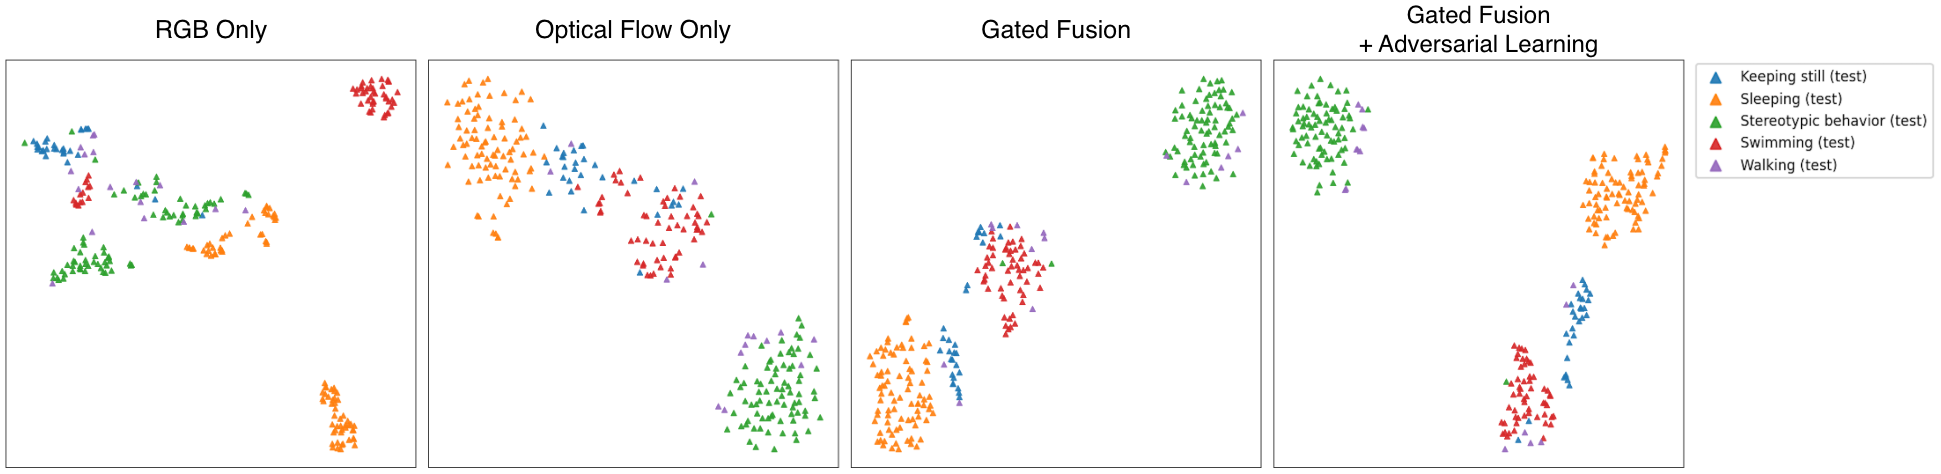
\includegraphics[width=0.9\linewidth]{image/tsne.png}
  \caption{ホッキョクグマデータセットにおける各手法の t-SNE 可視化結果．
    (a) RGB Only，(b) Flow Only，(c) Gated Fusion (w/o Adv)，(d) Proposed (Full)．
    提案手法では各行動クラスが明確に分離されたクラスタを形成している．}
  \label{fig:tsne_polar}
\end{figure}

RGB Only では各行動クラスのサンプルが混在しており，
明確なクラスタ構造が形成されていない．
一方，提案手法（Full）では「Swimming」「Walking」「Sleeping」などの
各行動クラスが明確に分離されたクラスタを形成しており，
クラス間の境界も明瞭である．

特に注目すべき点として，動物福祉の観点で重要な
「Stereotypic behavior（常同行動）」のクラスタが，
「Walking」と隣接しながらも明確に区別されている．
これは，常同行動が歩行の一種でありながらも，
その反復的なパターンが特徴空間上で識別可能であることを示唆しており，
異常行動の自動検知への応用可能性を示している．

\subsubsection{行動クラス間の誤分類分析}
詳細な誤分類の傾向を分析したところ，
一部の「Walking（歩行）」と「Stereotypic behavior（常同行動）」の間で
若干の混同が確認された．
これは，常同行動の多くが「同じ場所を行き来する歩行（ペーシング）」であるため，
動作特徴としての類似性が高いことに起因する．

しかし，敵対的学習導入前と比較すると，この分離性能は向上しており，
提案手法が行動間の微妙なニュアンスの違いを捉え始めていることがわかる．
今後は，行動の時間的パターン（周期性など）を考慮した特徴抽出により，
さらなる分離性能の向上が期待される．

\subsection{失敗事例の分析}
本手法における典型的な失敗事例として，
背景ノイズによる誤認識が挙げられる．

具体的には，「Swimming」行動において，
水面の反射や波紋が激しい場合に，
オプティカルフローが動物の動きではなく水面の動きを支配的に捉えてしまい，
特徴空間上で外れ値となるケースが確認された．
また，強風による植生の揺れが動物の動作と誤認識される事例も観察された．

これらの問題に対しては，
セグメンテーションによる前景・背景の分離や，
Attention 機構を用いた動物領域への選択的な特徴抽出など，
より高度な背景抑制技術の導入が必要である．


\section{実験2: アジアゾウ監視映像への汎化検証}
本節では，提案手法の汎化性能をさらに検証するため，
ホッキョクグマとは異なる動物種であるアジアゾウの監視映像に対する評価を行う．
これにより，提案手法が特定の動物種に依存しない汎用的な行動認識能力を持つかを確認する．

\subsection{定量評価結果}
アジアゾウ監視映像に対するクラスタリング性能を
表\ref{tab:clustering_results_elephant}に示す．

\begin{table}[t]
  \centering
  \caption{アジアゾウ監視映像に対する各手法のクラスタリング性能比較}
  \label{tab:clustering_results_elephant}
  \begin{tabular}{lcc}
    \hline
    手法 & ARI & NMI \\
    \hline \hline
    RGB Only & XXX & XXX \\
    Flow Only & XXX & XXX \\
    Gated Fusion (w/o Adv) & XXX & XXX \\
    \textbf{Proposed (Full)} & \textbf{XXX} & \textbf{XXX} \\
    \hline
  \end{tabular}
\end{table}

% TODO: 具体的な数値を入力後、以下の考察を更新
表\ref{tab:clustering_results_elephant}より，アジアゾウデータセットにおいても
提案手法が最も高い性能を示したことが確認された．
ただし，ホッキョクグマデータセット（ARI: 0.742）と比較すると，
全体的に性能が低下している．

\subsection{t-SNE による可視化}
アジアゾウデータセットにおける各手法の特徴空間を t-SNE により可視化した結果を
図\ref{fig:tsne_elephant}に示す．

\begin{figure}[t]
  \centering
  % TODO: t-SNE画像のパスを指定
  % \includegraphics[width=0.9\linewidth]{image/tsne_elephant.png}
  \caption{アジアゾウデータセットにおける各手法の t-SNE 可視化結果．
    ホッキョクグマと比較してクラスタの分離が不明瞭である．}
  \label{fig:tsne_elephant}
\end{figure}

ホッキョクグマの結果と比較すると，各行動クラスのクラスタ分離が
相対的に不明瞭であることが確認された．
特に，一部の行動カテゴリ間で重複が見られ，
これが定量指標の低下に寄与していると考えられる．

\subsection{ホッキョクグマとの比較分析}
表\ref{tab:comparison_polar_elephant}に，ホッキョクグマとアジアゾウの
両データセットにおける提案手法の性能比較を示す．

\begin{table}[t]
  \centering
  \caption{ホッキョクグマとアジアゾウにおける提案手法の性能比較}
  \label{tab:comparison_polar_elephant}
  \begin{tabular}{lcc}
    \hline
    データセット & ARI & NMI \\
    \hline \hline
    ホッキョクグマ & 0.742 & 0.728 \\
    アジアゾウ & XXX & XXX \\
    \hline
  \end{tabular}
\end{table}

アジアゾウデータセットにおいて性能が低下した主な要因として，
以下の点が考えられる：

\paragraph{複数個体の存在}
ホッキョクグマのデータセットでは基本的に単一個体が撮影されているのに対し，
アジアゾウのデータセットでは2頭のゾウが同一フレーム内に存在することがある．
現在の手法はクリップ全体から特徴を抽出するため，
複数個体が異なる行動を同時に行っている場合，
それらが混合された特徴が抽出され，行動識別が困難になる．

\paragraph{体サイズと動作の特性}
ゾウはホッキョクグマと比較して体が大きく，動作が緩慢である傾向がある．
そのため，オプティカルフローによる運動特徴の抽出において，
動作の微細な差異を捉えにくい可能性がある．
また，長い鼻（trunk）の動きが行動とは独立に発生するため，
ノイズとして作用している可能性もある．

\paragraph{行動カテゴリの曖昧性}
ゾウの行動は，ホッキョクグマと比較して境界が曖昧なものが多い可能性がある．
例えば，「立っている」状態と「ゆっくり歩いている」状態の遷移が
連続的であり，明確な区別が困難な場合がある．


\section{実験3: ソースドメイン内での行動分類}
本節では，学習に使用した Animal Kingdom データセットのテストセットに対する
提案手法の性能を評価する．
これにより，提案手法がソースドメイン内（In-domain）において
基本的な行動認識能力を維持しているかを確認する．

\subsection{定量評価結果}
Animal Kingdom テストセットに対するクラスタリング性能を
表\ref{tab:clustering_results_ak}に示す．

\begin{table}[t]
  \centering
  \caption{Animal Kingdom テストセットに対する各手法のクラスタリング性能比較}
  \label{tab:clustering_results_ak}
  \begin{tabular}{lcc}
    \hline
    手法 & ARI & NMI \\
    \hline \hline
    RGB Only & 0.412 & 0.486 \\
    Flow Only & 0.385 & 0.451 \\
    Gated Fusion (w/o Adv) & 0.523 & 0.572 \\
    \textbf{Proposed (Full)} & \textbf{0.548} & \textbf{0.591} \\
    \hline
  \end{tabular}
\end{table}

ソースドメイン内での評価では，ターゲットドメインとは異なる傾向が観察された．
具体的には，RGB Only と Flow Only の性能差が小さく，
両者ともに中程度の性能を示した．
これは，学習データと評価データが同一分布に属するため，
外観特徴もドメインシフトの影響を受けにくいためと考えられる．

提案手法（Full）は ARI 0.548 を達成し，
Gated Fusion (w/o Adv) と比較してわずかながら性能が向上した．
敵対的学習の効果はターゲットドメインほど顕著ではないが，
ソースドメイン内においても性能を維持しつつ，
汎化性能を大幅に向上させることに成功していると言える．

\subsection{特徴空間におけるクラス間距離の分析}

学習された特徴空間における各行動クラスの分離性をより詳細に評価するため，
特徴空間上でのクラス間およびクラス内におけるサンプルのユークリッド距離の平均と分散を算出した．
表\ref{tab:distance_mean}に距離の平均値を，表\ref{tab:distance_var}に距離の分散を示す．
対角成分は同一クラス内のサンプルペア間の距離（クラス内距離），
非対角成分は異なるクラス間のサンプルペア間の距離（クラス間距離）を表す．

\begin{table}[t]
  \centering
  \caption{各行動クラス間の特徴空間上での距離平均（対角成分はクラス内距離）}
  \label{tab:distance_mean}
  \resizebox{\columnwidth}{!}{
  \begin{tabular}{lccccccc}
    \hline
     & Attending & Eating & Jumping & Keeping still & Running & Sensing & Walking \\
    \hline \hline
    Attending & 0.755 & 0.833 & 0.861 & 0.786 & 1.021 & 0.834 & 0.888 \\
    Eating & 0.833 & \textbf{0.672} & 1.020 & 0.849 & \textbf{1.120} & 0.892 & 0.903 \\
    Jumping & 0.861 & 1.020 & \textbf{0.648} & 0.831 & 0.762 & 0.872 & 0.813 \\
    Keeping still & 0.786 & 0.849 & 0.831 & 0.680 & 0.942 & 0.763 & \textit{0.746} \\
    Running & 1.021 & \textbf{1.120} & 0.762 & 0.942 & \textbf{0.640} & 0.981 & 0.804 \\
    Sensing & 0.834 & 0.892 & 0.872 & 0.763 & 0.981 & 0.722 & 0.812 \\
    Walking & 0.888 & 0.903 & 0.813 & \textit{0.746} & 0.804 & 0.812 & \textbf{0.648} \\
    \hline
  \end{tabular}
  }
\end{table}

\begin{table}[t]
  \centering
  \caption{各行動クラス間の特徴空間上での距離分散}
  \label{tab:distance_var}
  \resizebox{\columnwidth}{!}{
  \begin{tabular}{lccccccc}
    \hline
     & Attending & Eating & Jumping & Keeping still & Running & Sensing & Walking \\
    \hline \hline
    Attending & 0.084 & 0.061 & 0.066 & 0.054 & 0.069 & 0.054 & 0.066 \\
    Eating & 0.061 & 0.069 & 0.077 & 0.063 & 0.086 & 0.058 & 0.100 \\
    Jumping & 0.066 & 0.077 & 0.084 & 0.059 & 0.064 & 0.054 & 0.067 \\
    Keeping still & 0.054 & 0.063 & 0.059 & 0.085 & 0.103 & 0.054 & 0.079 \\
    Running & 0.069 & 0.086 & 0.064 & 0.103 & \textbf{0.125} & 0.084 & \textbf{0.150} \\
    Sensing & 0.054 & 0.058 & 0.054 & 0.054 & 0.084 & 0.080 & 0.070 \\
    Walking & 0.066 & 0.100 & 0.067 & 0.079 & \textbf{0.150} & 0.070 & 0.102 \\
    \hline
  \end{tabular}
  }
\end{table}

表\ref{tab:distance_mean}の結果から，以下の傾向が読み取れる．
まず，対角成分（クラス内平均距離）は，非対角成分（クラス間平均距離）と比較して全体的に小さな値をとっている．
特に「Running」「Jumping」「Walking」などの動作を伴うクラスにおいて，
0.640--0.648程度と低い値を示しており，
これらの行動が特徴空間上で凝集度の高いクラスタを形成していることがわかる．

一方で，「Eating」と「Running」の間の平均距離は1.120と最も大きく，
静的な要素を含む採食行動と，激しい動きを伴う走行行動が
明確に区別されていることを示している．
これに対し，「Keeping still（静止）」と「Walking（歩行）」の間の距離は0.746と，
異種クラス間では比較的小さい値となった．
これは，ゆっくりとした歩行や立ち止まりかけた状態など，
両者の境界線上にある動作が特徴空間上でも近接していることを示唆しており，
前述の誤分類の傾向とも整合する．

また，表\ref{tab:distance_var}の分散に注目すると，
「Running」に関連する項で分散が大きい傾向が見られた（クラス内分散：0.125，Walkingとのクラス間分散：0.150）．
これは，「Running」という行動クラスの内部に多様な速度や姿勢の変化が含まれていることや，
「Walking」との境界が曖昧なサンプルが存在することを示している．

\subsection{ゲーティングパラメータの分析}
提案手法の Gated Fusion 機構が，
実際にどのように外観・運動特徴を統合しているかを分析するため，
学習過程におけるゲーティングパラメータ $\boldsymbol{\alpha}$ の変化を調査した．
図\ref{fig:alpha_stats}に，学習エポックごとの $\boldsymbol{\alpha}$ の平均値，最大値，最小値，および標準偏差の推移を示す．

\begin{figure}[t]
  \centering
  \begin{minipage}{0.48\linewidth}
    \centering
    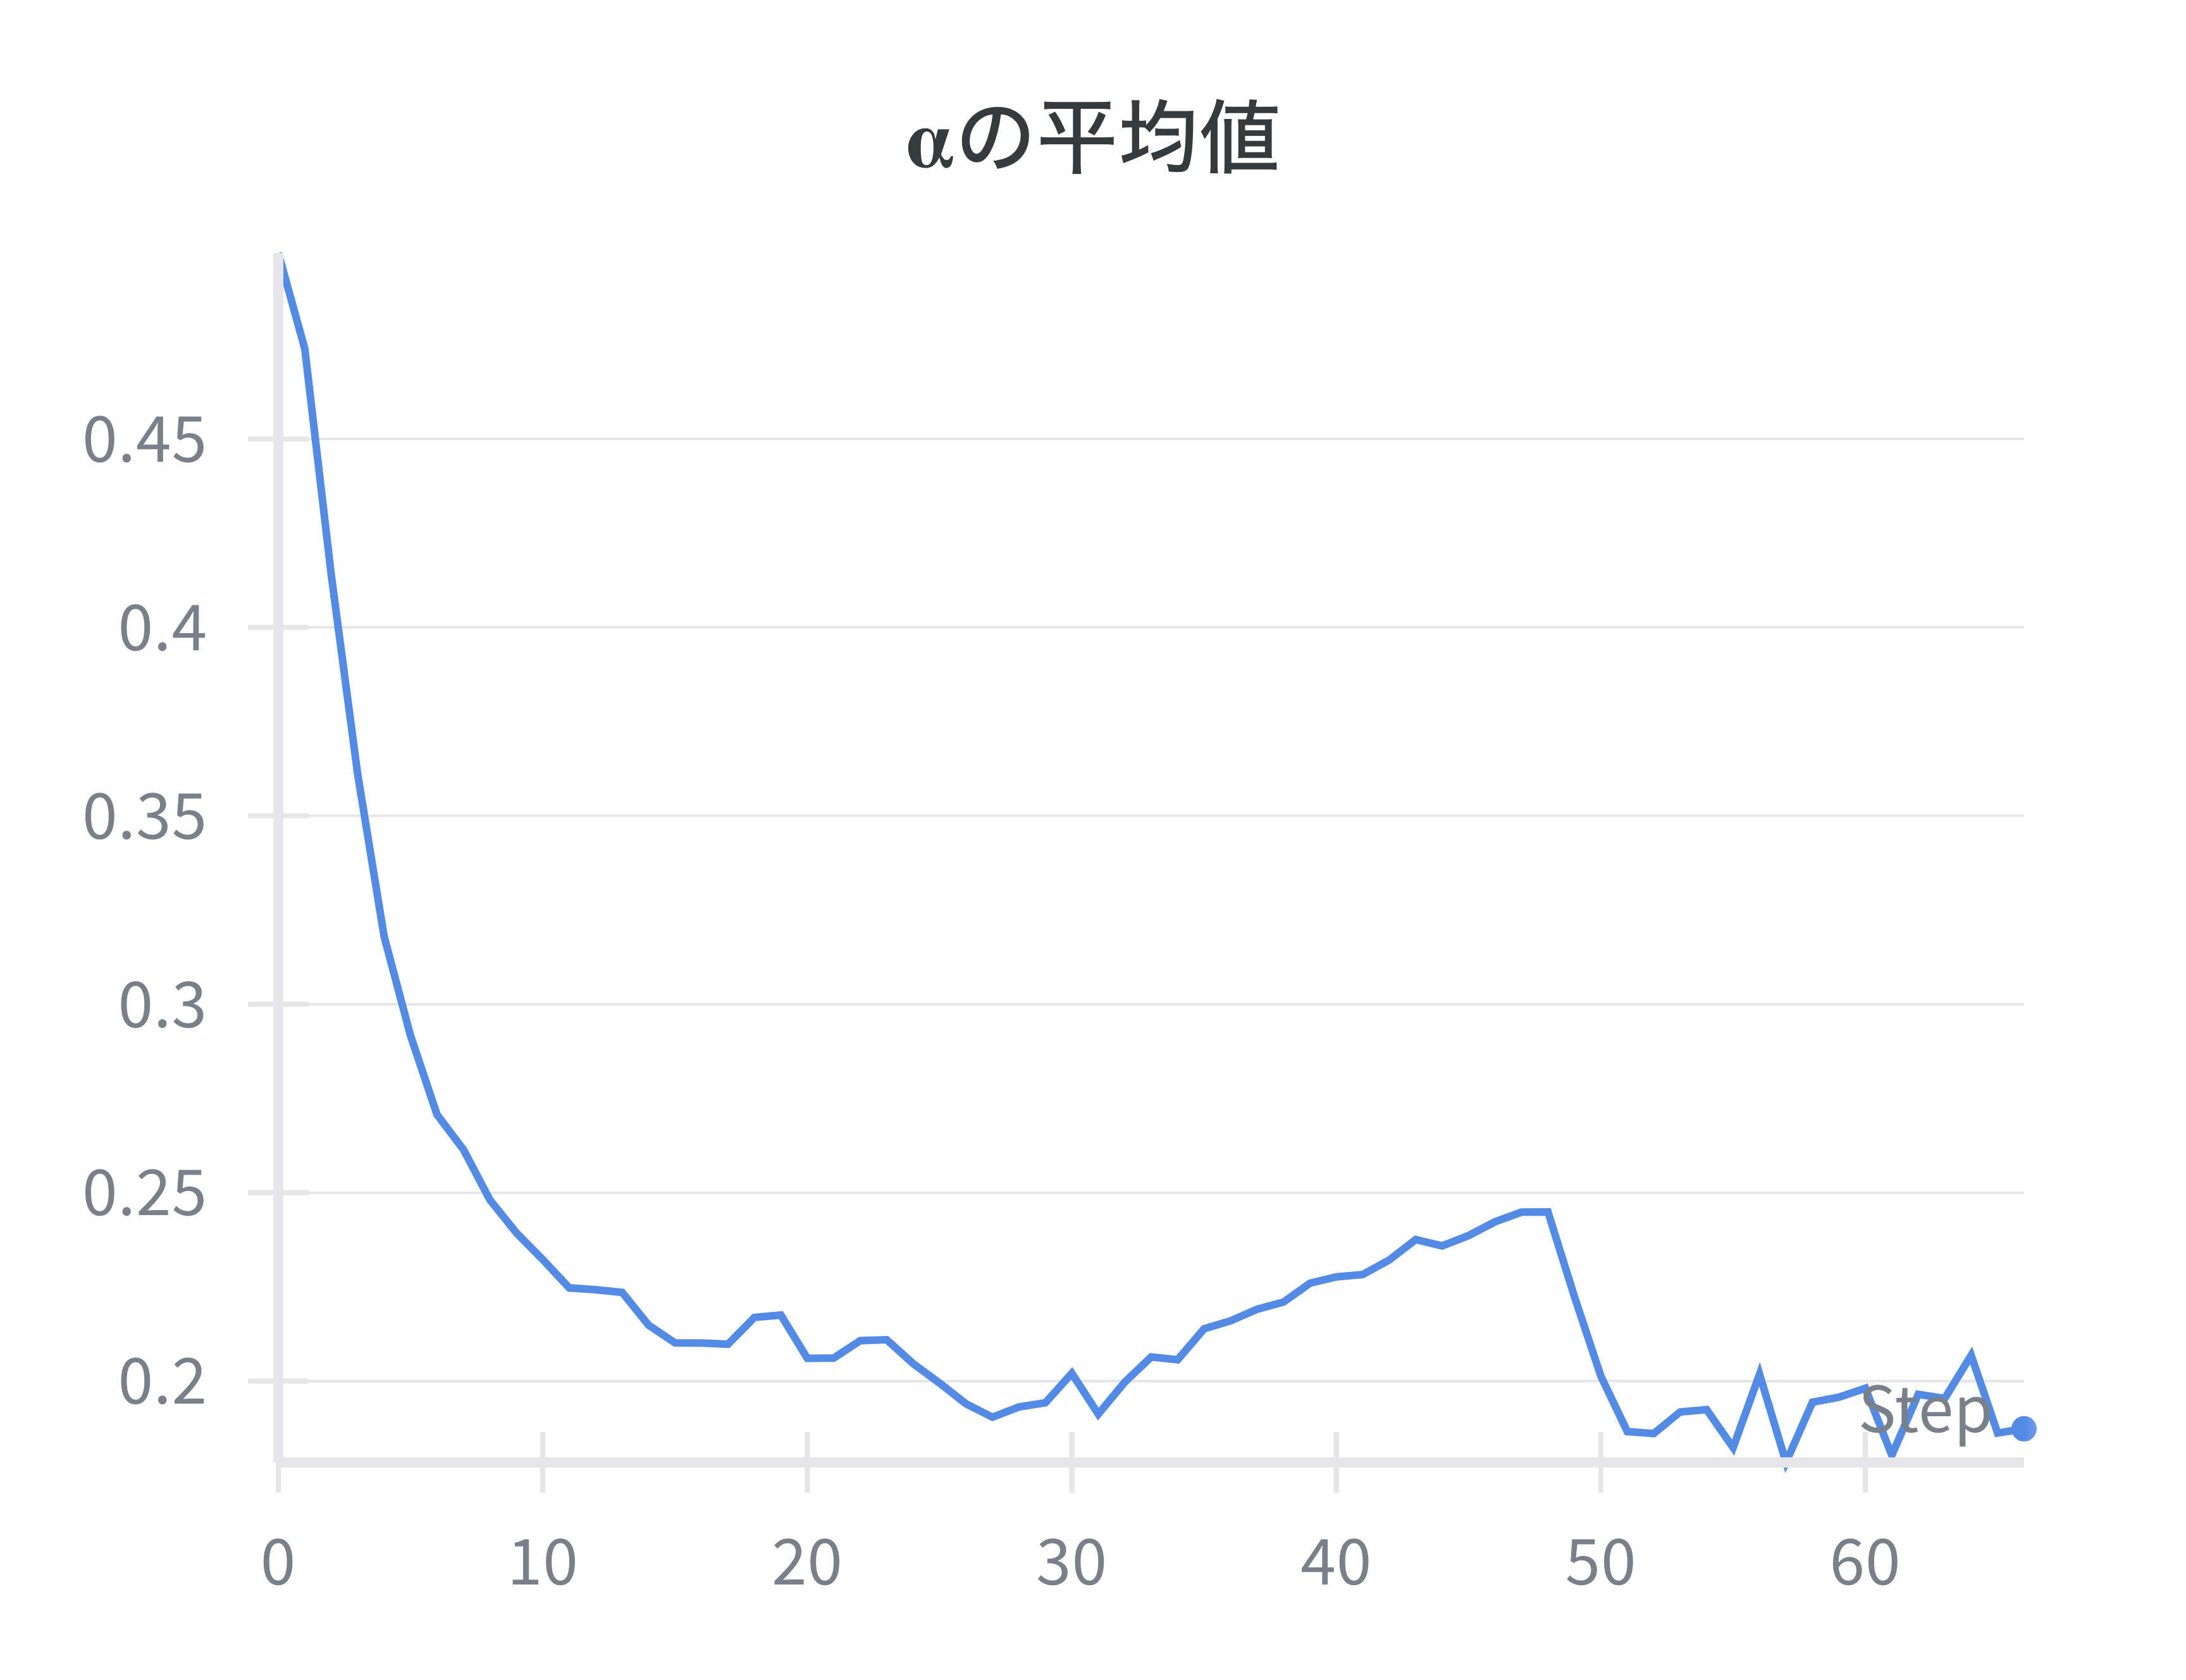
\includegraphics[width=\linewidth]{image/alpha_mean.png}
    \subcaption{Mean of $\boldsymbol{\alpha}$}
  \end{minipage}
  \hfill
  \begin{minipage}{0.48\linewidth}
    \centering
    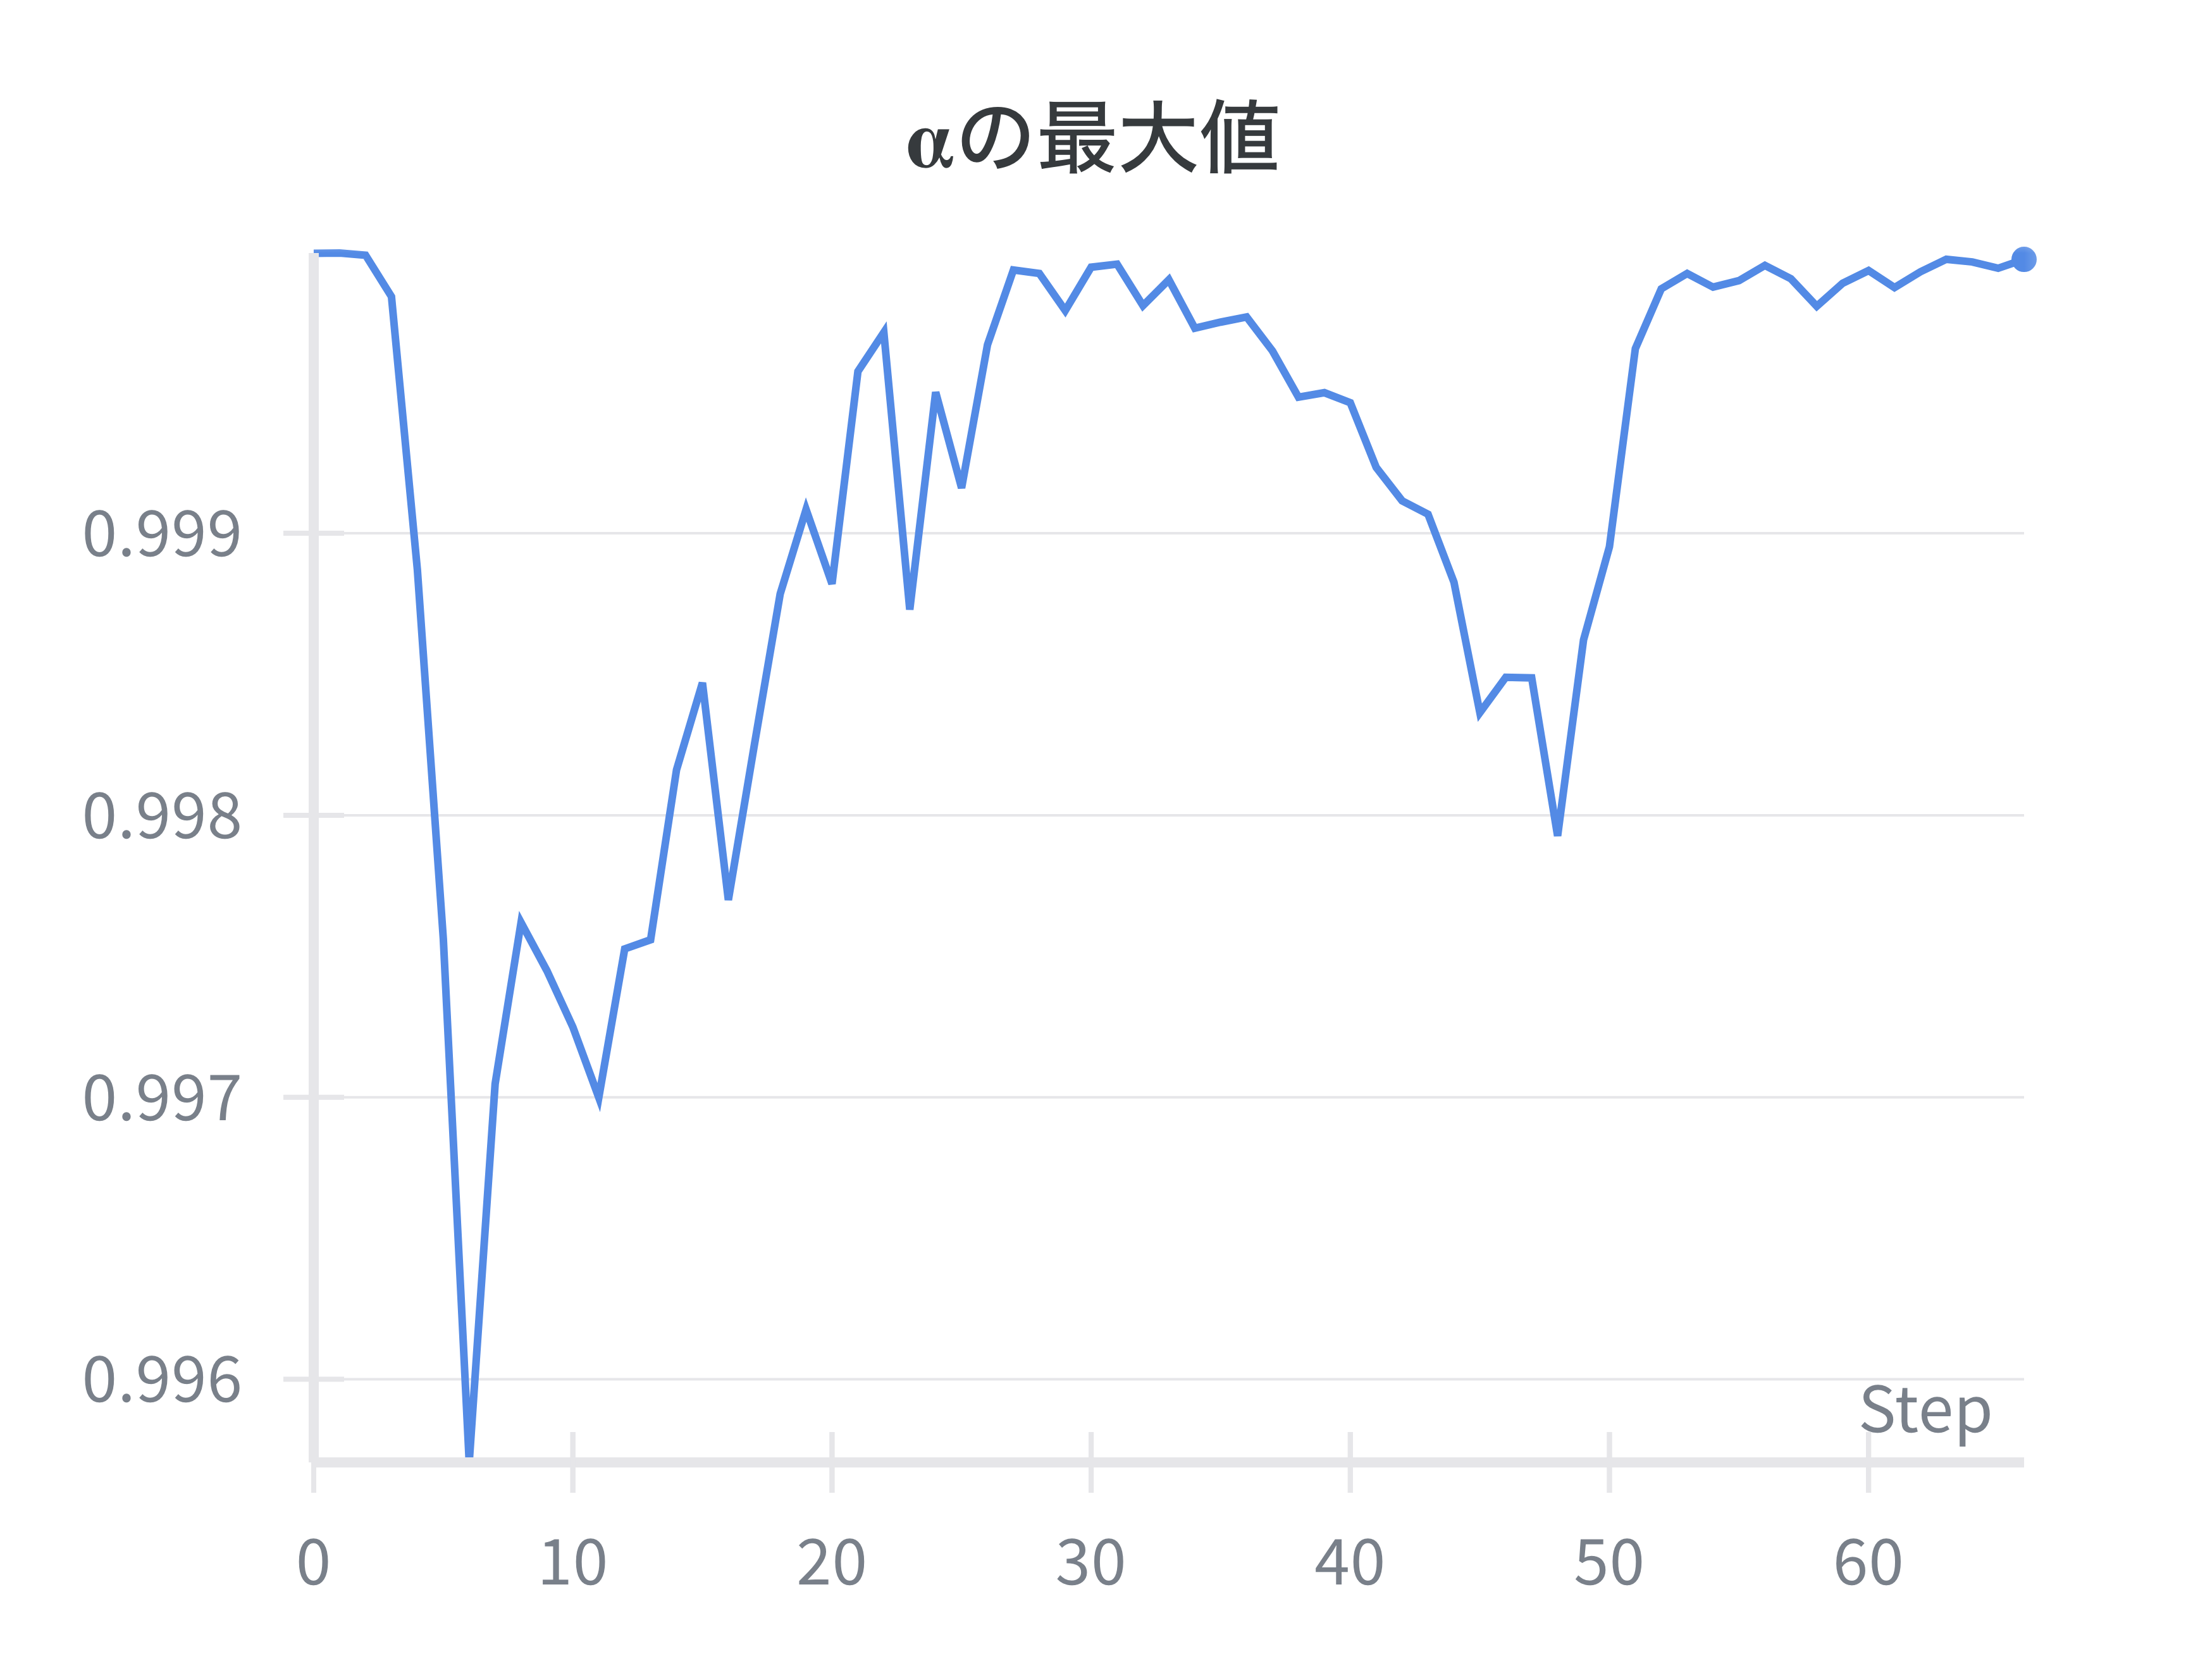
\includegraphics[width=\linewidth]{image/alpha_max.png}
    \subcaption{Max of $\boldsymbol{\alpha}$}
  \end{minipage}
  \vspace{1em} \\ 
  \begin{minipage}{0.48\linewidth}
    \centering
    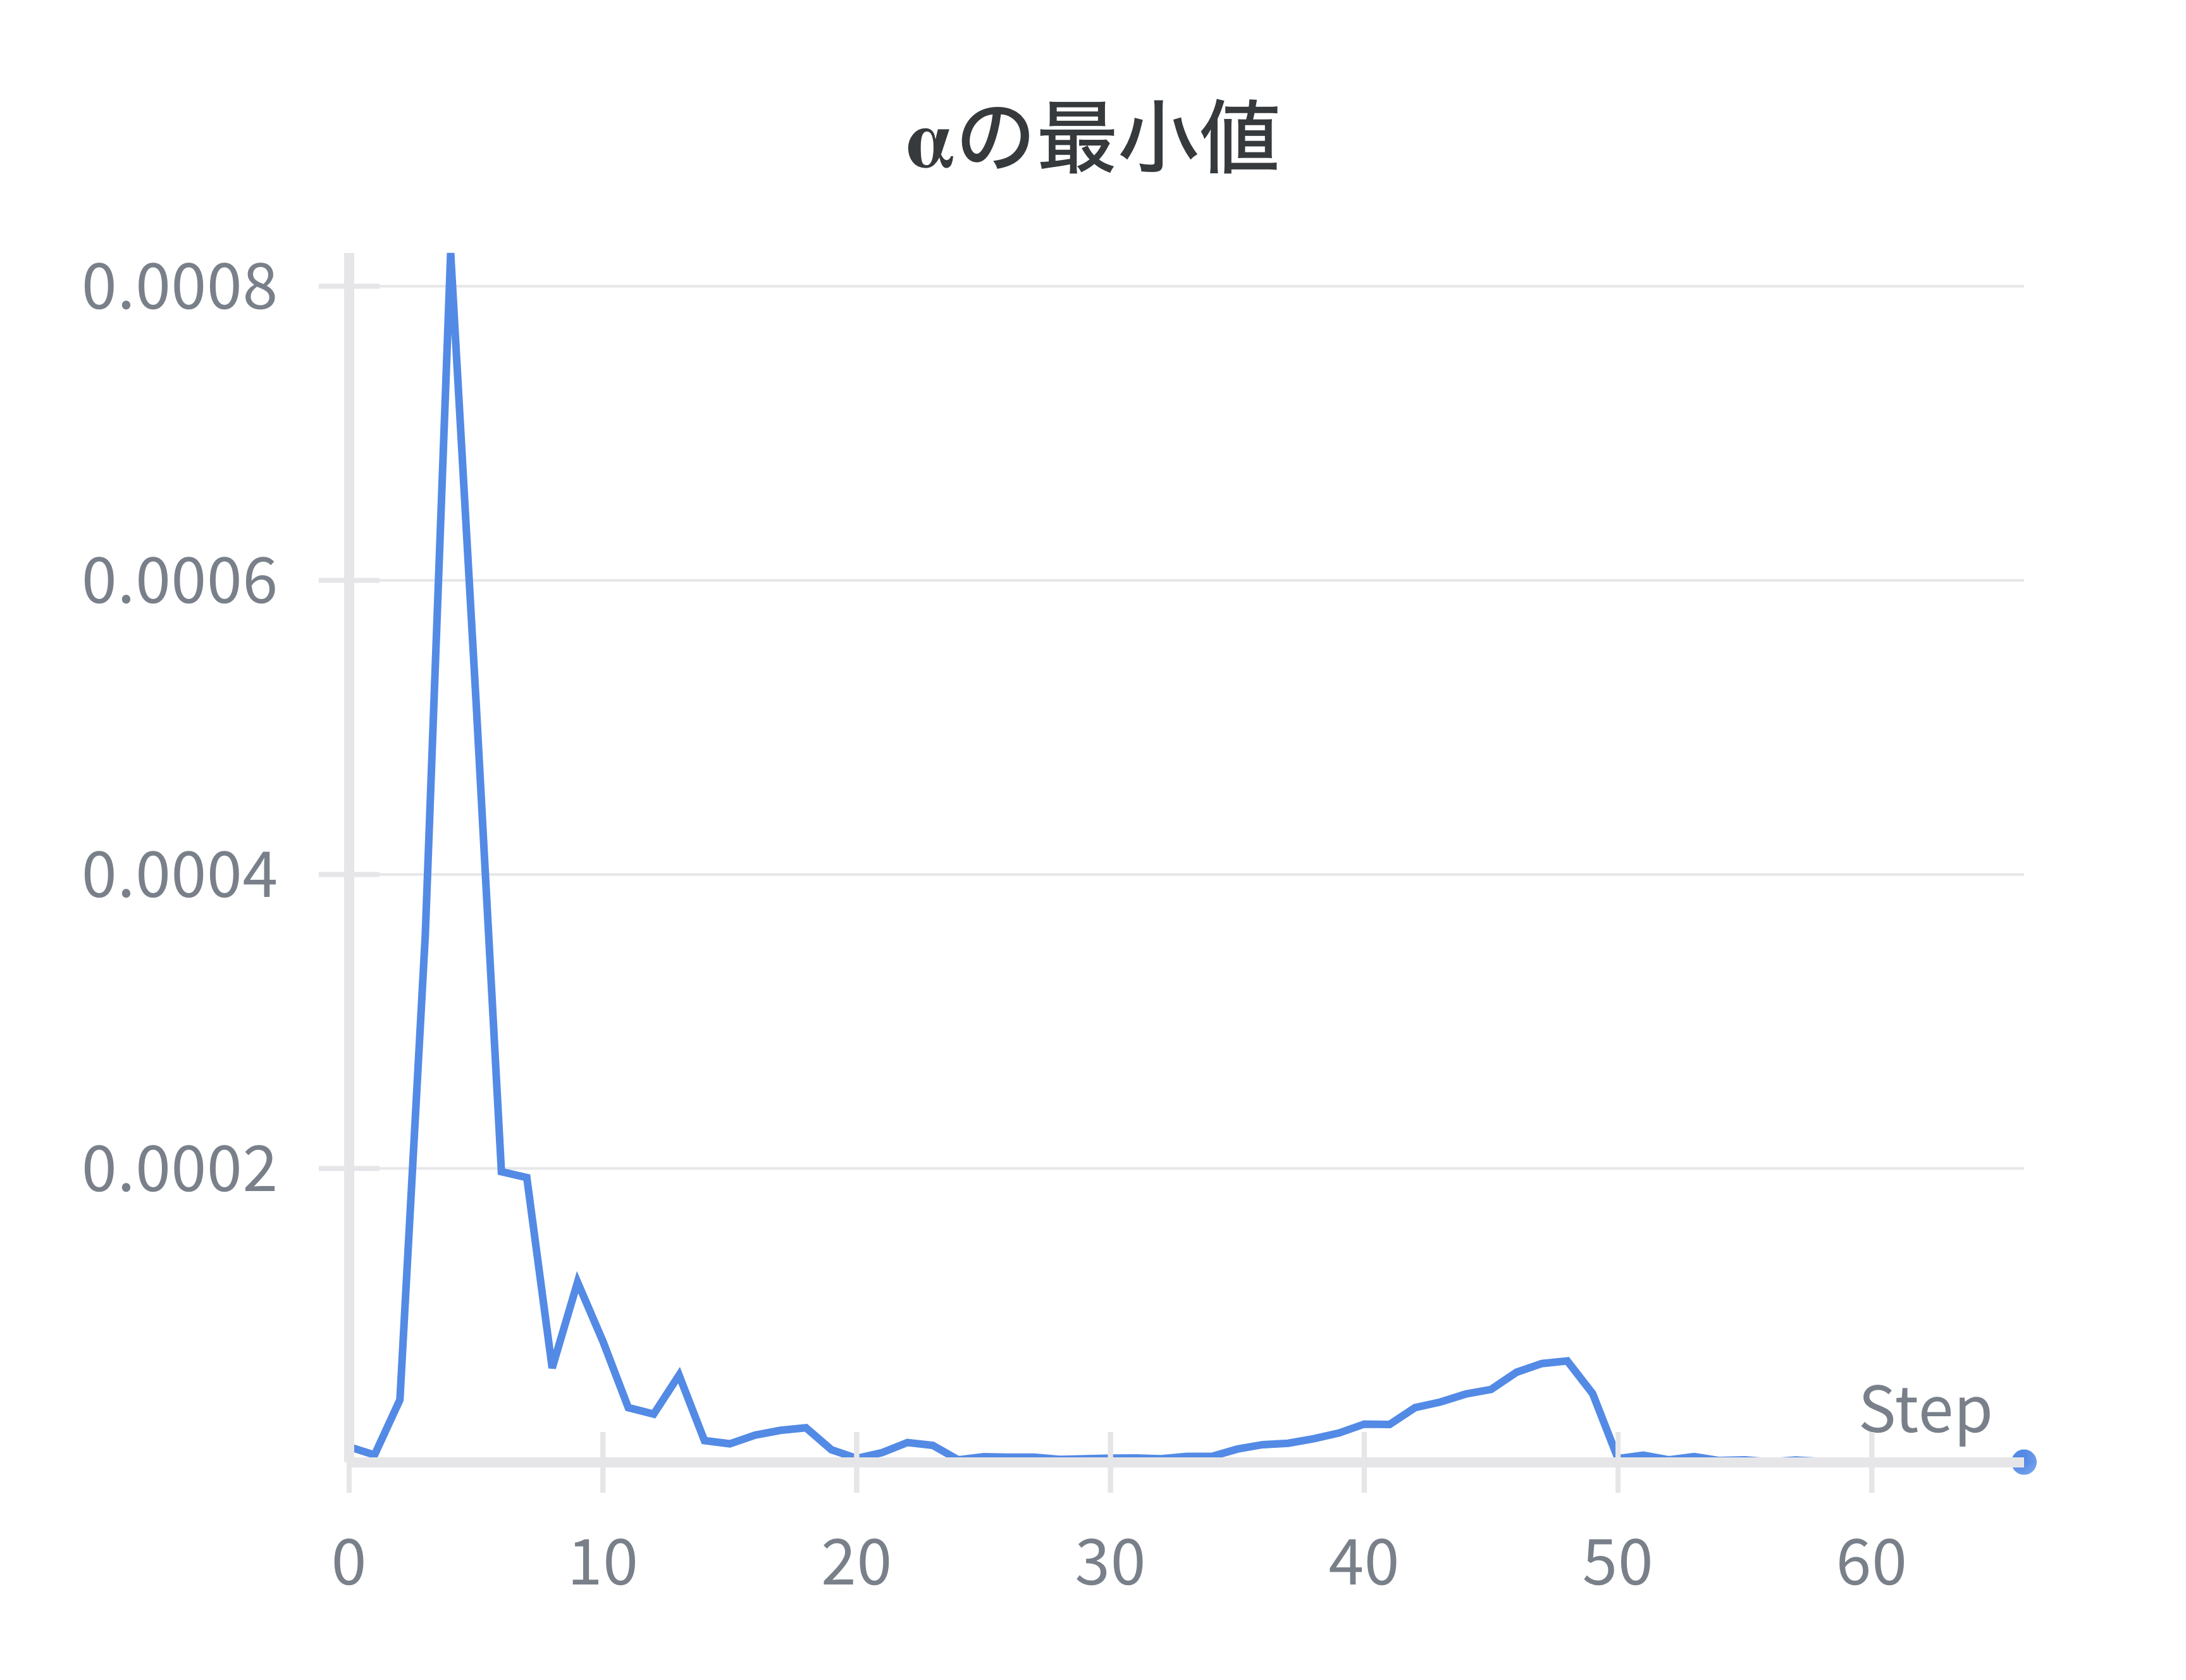
\includegraphics[width=\linewidth]{image/alpha_min.png}
    \subcaption{Min of $\boldsymbol{\alpha}$}
  \end{minipage}
  \hfill
  \begin{minipage}{0.48\linewidth}
    \centering
    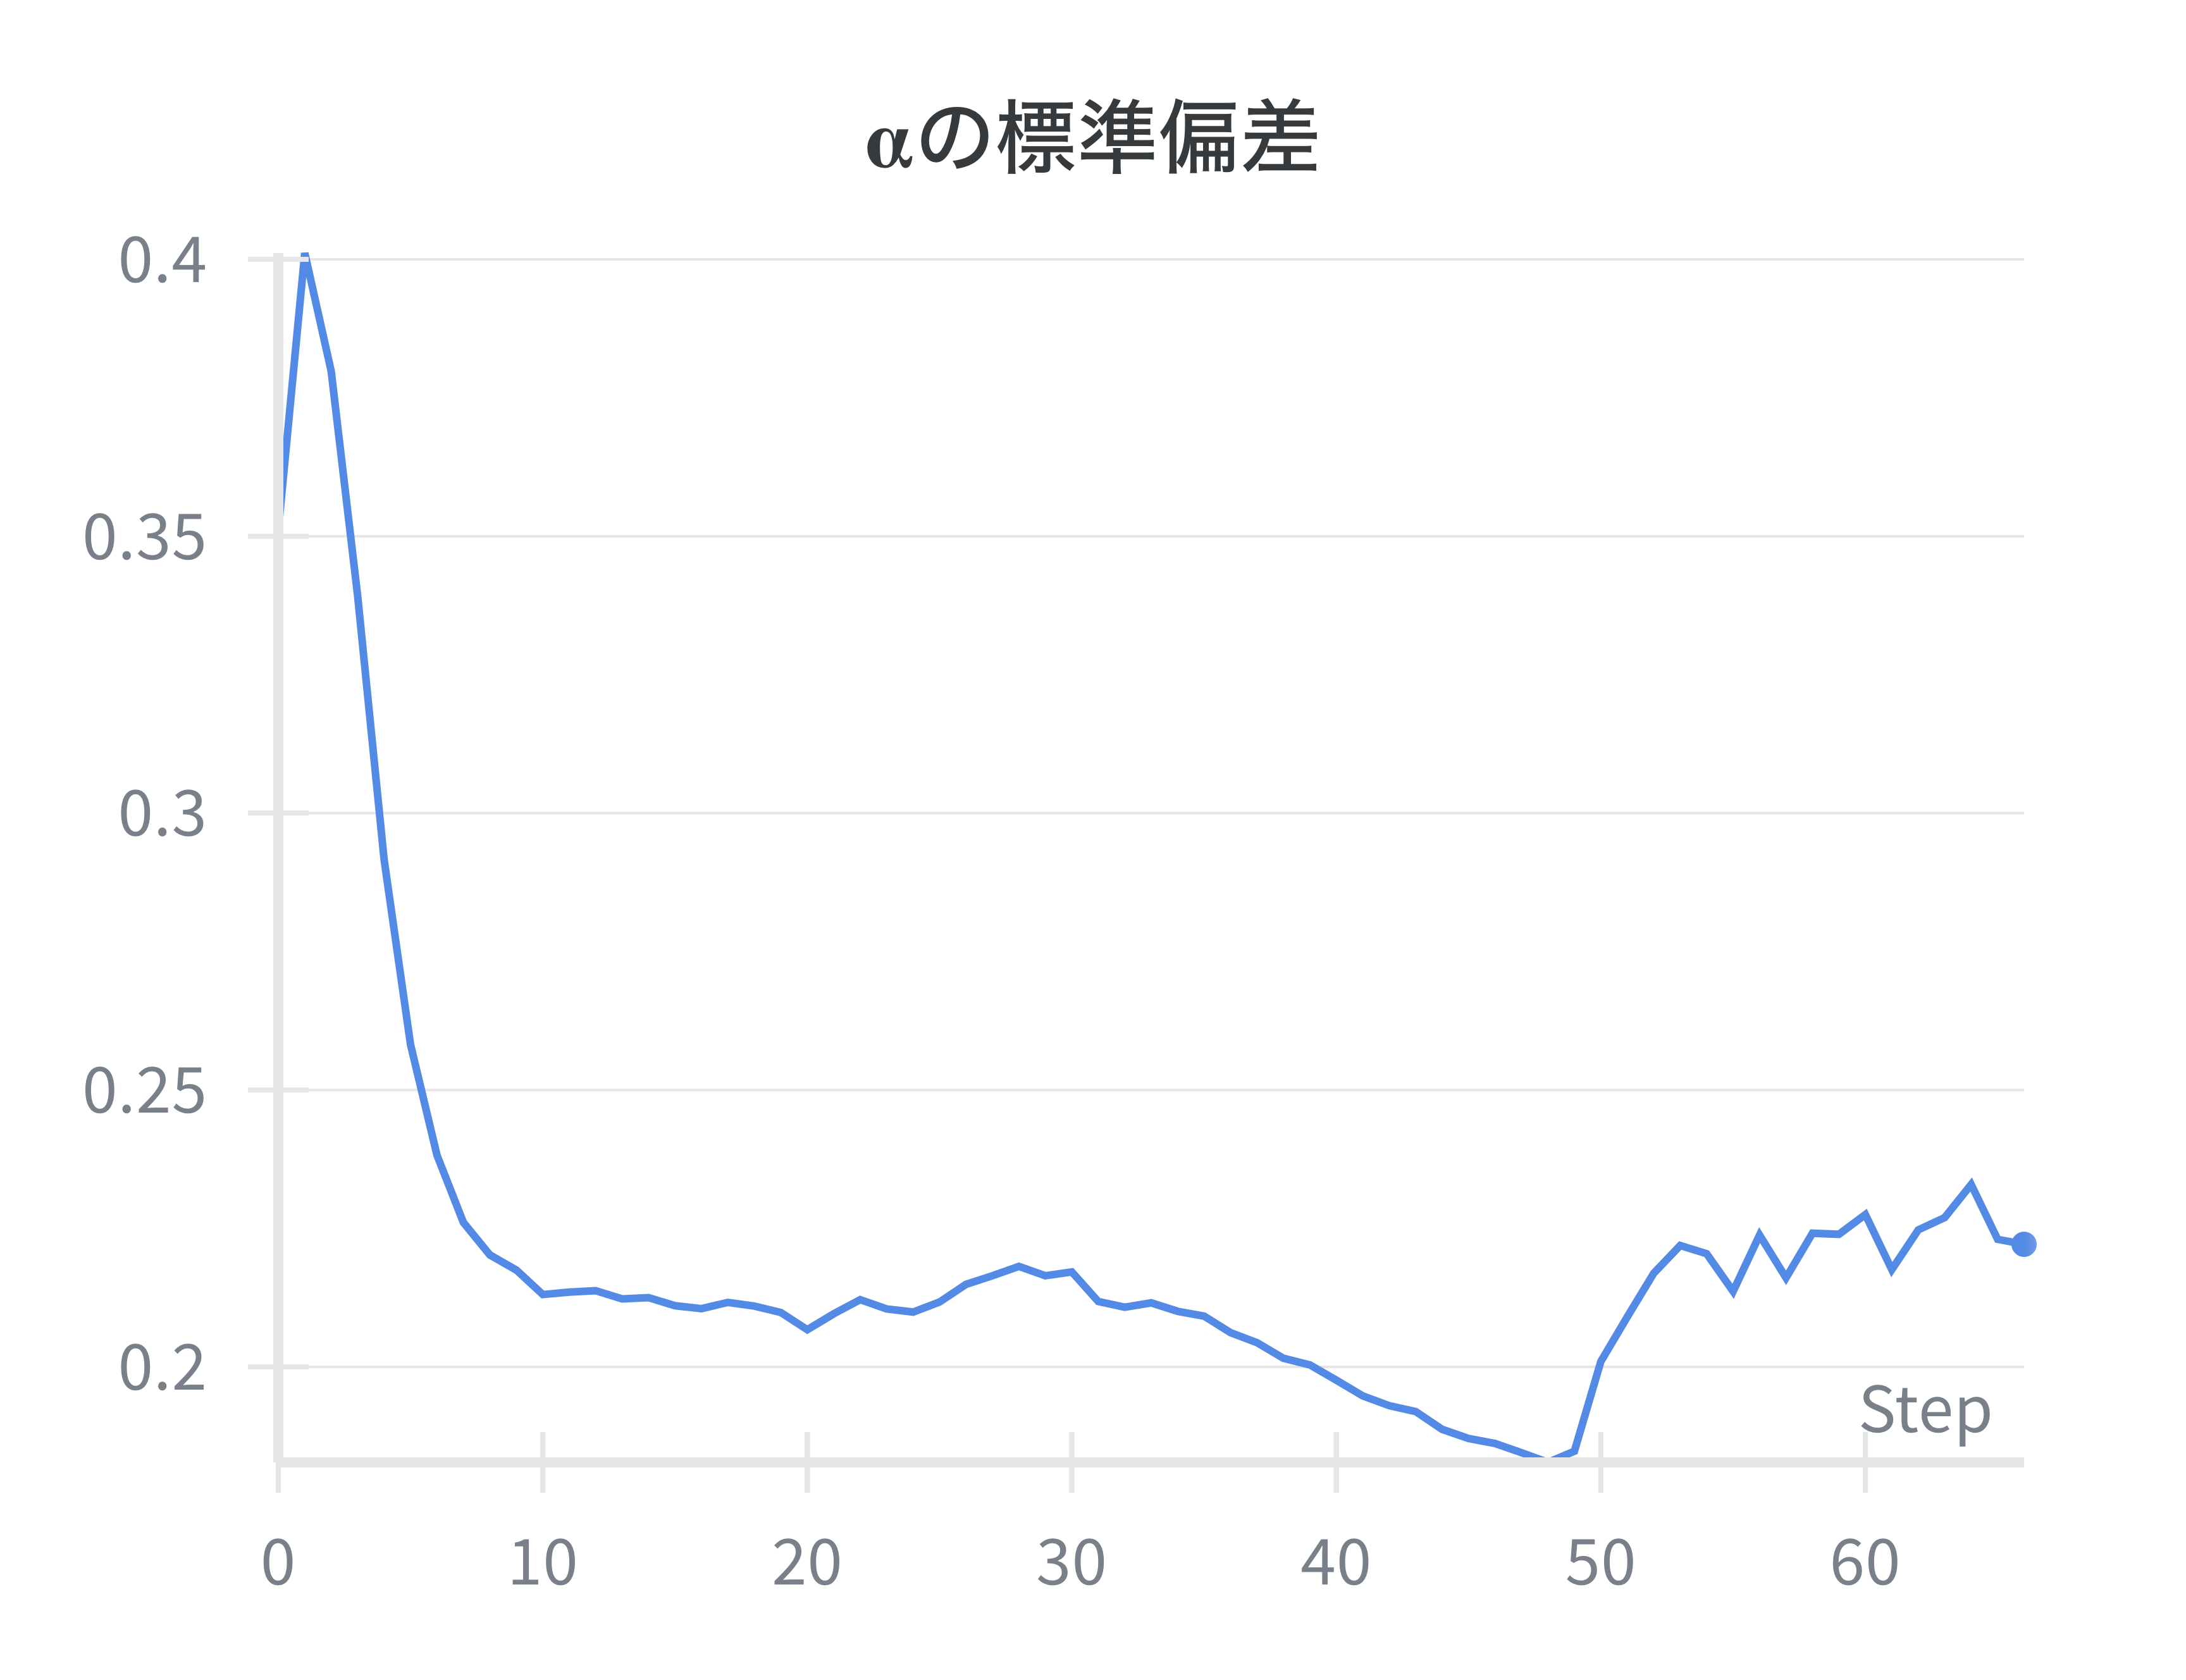
\includegraphics[width=\linewidth]{image/alpha_std.png}
    \subcaption{Std of $\boldsymbol{\alpha}$}
  \end{minipage}
  \caption{
    Gated Fusion パラメータ $\boldsymbol{\alpha}$ の学習過程における統計量の推移．
    (a) 平均値は約0.2に収束し，全体的には外観特徴（$1-\boldsymbol{\alpha}$）が重視されていることを示す．
    (b) 最大値は高い値（約1.0）を維持しており，一部の特徴次元では運動特徴（$\boldsymbol{\alpha}$）が支配的であることを示す．
    (c) 最小値は0付近に収束している．
    (d) 標準偏差は学習の進行とともに減少し，パラメータが安定していることを示す．
  }
  \label{fig:alpha_stats}
\end{figure}

分析の結果，以下の特徴が明らかになった：
\begin{enumerate}
  \item \textbf{平均値の収束と外観特徴の優位性}：
    $\boldsymbol{\alpha}$ の平均値（図\ref{fig:alpha_stats}(a)）は学習初期の約0.45から徐々に減少し，約0.2付近で収束している．
    これは，ソースドメイン（Animal Kingdom）においては，
    全体の特徴次元の約80\%が外観特徴（RGB）によって支配されていることを意味する．
    野生動物のドキュメンタリー映像は背景や環境が多様ではあるものの，
    動物の姿勢やテクスチャといった外観情報が依然として強力な手がかりとなっている．

  \item \textbf{局所的な運動特徴の選択}：
    一方で，$\boldsymbol{\alpha}$ の最大値（図\ref{fig:alpha_stats}(b)）は学習全体を通じて高い値を維持した．
    これは，全体的には外観重視でありながらも，
    特定の特徴次元においては運動特徴（オプティカルフロー）が支配的に利用されていることを示している．

  \item \textbf{学習の安定性}：
    $\boldsymbol{\alpha}$ の標準偏差（図\ref{fig:alpha_stats}(d)）は学習が進むにつれて減少しており，
    各次元の重み付けが学習とともに安定した値に収束していることが確認できる．
    
  \item \textbf{適応的統合の実態}：
    この結果は，Gated Fusion が単に両モダリティを平均化するのではなく，
    「基本的には外観情報を使いつつ，必要な情報のみを運動特徴から選択的に取り入れる」
    という洗練された統合を実現していることを示唆している．
    この選択的な運動情報の利用が，
    ドメインシフトの大きいターゲットドメイン（シロクマやゾウ）において，
    背景不変な行動特徴として機能し，
    高い汎化性能の達成に寄与したと考えられる．
\end{enumerate}
